\documentclass[12pt]{article}
\usepackage{graphicx} % Required for inserting images
\usepackage{ragged2e}  % Enables justification
\usepackage{geometry}
\usepackage{caption}
\usepackage{subcaption}
\usepackage[x11names]{xcolor}
\usepackage{minted}
\usepackage{xparse}
\usepackage{wrapfig}
\usepackage{amsmath}
\usepackage{float}
\usepackage[
    backend=biber,
    style=numeric-comp,
    sorting=none
]{biblatex}
\usepackage{hyperref}
\usepackage{soul}
\usepackage{mathtools}
\usepackage{amssymb}
\usepackage{cancel}
\usepackage{dirtytalk}
\usepackage{scrextend}
\usepackage{multicol}
\usepackage{booktabs}

\addbibresource{references.bib}

\hypersetup{
    colorlinks=true,
    linkcolor=blue,
    citecolor=SpringGreen4,
    filecolor=magenta,      
    urlcolor=cyan,
    pdftitle={An Exploration of Statistical Methods in Determining the Gaussianity of LIGO Detector Data},
    pdfpagemode=FullScreen,
    }

\definecolor{shellbackground}{rgb}{0.95,0.95,0.92}

\geometry{
letterpaper,
% left=0.75in,
% right=0.75in,
left=0.8in,
right=0.8in,
top=0.8in,
bottom=0.8in
}

\begin{document}

\begin{titlepage}
  \vspace*{1cm}
  \centering
  {\LARGE \textbf{University of Massachusetts Dartmouth}}\\[1.5cm]
  {\Large \textbf{Department of Mathematics}}\\[2cm]
  {\huge \textbf{An Exploration of Statistical Methods in Determining the Gaussianity of LIGO Detector Data}}\\[3cm]
  {\Large A project in}\\[0.2cm]
  {\Large Data Science}\\[0.2cm]
  {\Large by}\\[0.2cm]
  {\Large Ashish Thomas Mathew}\\[2.5cm]
  {\Large Submitted in Partial Fulfillment of the}\\[0.5cm]
  {\Large Requirements for the Degree of}\\[0.5cm]
  {\Large Master of Science}\\[2cm]
  {\large \textbf{May, 2025}}
  \vfill
\end{titlepage}

\clearpage  % Ensure it starts on a new page
\normalfont % Reset to normal font (removes centering effects)
\raggedright % Ensure left alignment (prevents centering issues)

\begin{center}
    \Large \textbf{Abstract}  % Title formatting
\end{center}

\justifying

\noindent The Advanced Laser Interferometer Gravitational-wave Observatory (LIGO) is one of the most sophisticated instruments ever built, capable of measuring motion 10,000 times smaller than a proton, and was the first device to detect a Gravitational Wave (GW) event. Due to its high sensitivity, a common issue is its susceptibility to glitches: transient, non-Gaussian noise bursts occurring at a high enough rate to contaminate the time series data obtained from the detector. The current methods to detect and study glitches, though highly effective for analyzing the strain data during the detection run, prove to be slow when working with a large throughput of detector data. Here we study a few possible statistical approaches to detecting these glitches in the time-amplitude domain. By sampling the strain data, conditioning it, and employing tests of normality, mainly the Shapiro-Wilk test, the Kolmogorov-Smirnov test, and the Anderson-Darling test, we gauge their effectiveness in determining the Gaussianity of a sample time-series strain data from the detector. The alternate hypothesis of these tests, i.e., the sample belonging to a non-Gaussian distribution, indicates the presence of a glitch or a signal. The results of this experiment explore in detail the viability of these tests as efficient alternatives to the current solutions used in detecting a glitch or astrophysical event in a time series signal.

\section{Introduction}\label{Introduction}

\noindent Nearly a century after Einstein's prediction of the existence of Gravitational Waves (GWs) in 1916, the first direct gravitational wave detection was achieved by the Advanced Laser Interferometer Gravitational-Wave Observatory (aLIGO) and Virgo collaboration during the binary black hole merger event GW150914 on September 14, 2015. The LIGO Livingston (L1) interferometer underwent several upgrades following this run - effectively a massive redesign - enhancing its sensitivity by 15\% to 25\% \cite{grant_advanced_2016}. This improvement was evident during the O2 observing run during which L1, in conjunction with its Hanford (H1) counterpart and Virgo (V1), detected eleven new gravitational wave signals \cite{collaboration_gwtc-1_2019}. Subsequently, during the O3 run, all three detectors operated at their best possible sensitivity, leading to the first single-detector GW detection, GW190425, achieved by LIGO Livingston \cite{abbott_gwtc-2_2021}. There have been over 90 GW events recorded at a high level of confidence since the LIGO-Virgo collaboration's inception to date.

\medskip
\noindent A consequence of these detectors' sensitivities is their susceptibility to noise. During observation runs, various noise sources, such as seismic noise, suspension thermal noise, and sensing noise, affect the data collected by the interferometers. All these sources collectively produce time series signals which can be treated as stochastic processes with their corresponding joint probability distributions and statistical properties \cite{collaboration_guide_2020}. In the absence of astronomical signals or glitches, the probability distribution of the noise follows a normal distribution, also known as \textit{Gaussian} noise. In the event of a Gravitational wave or any other signal, the noise exhibits a high signal-to-noise ratio (SNR), making it \textit{non-Gaussian}.

\medskip
\noindent Among these noise sources, the most problematic are \textbf{glitches}: transient events caused by non-astrophysical phenomena such as anthropogenic noise, weather conditions, or instrument malfunctions \cite{collaboration_guide_2020, collaboration_characterization_2016}. Glitches manifest as localized bursts of excess power in interferometer time series data and often do not have well-defined sources. They can occur at energy levels and frequencies that overlap with GW signals, thereby mimicking them and increasing the number of false positive detections. During the first half of the third observing run (O3a) LIGO Hanford and Livingston recorded glitches rates of $0.29\text{ min}^{-1}$ and $1.10\text{ min}^{-1}$ respectively, which rose to $0.32\text{ min}^{-1}$ and $1.17\text{ min}^{-1}$ during the second half (O3b) \cite{collaboration_gwtc-3_2023}. Of the 90 candidate events detected in this run, 17 had a probability of astronomical origin ($p_\text{astro}$) below 0.5, suggesting significant ambiguity about their origin. A notable example of glitches posing such an issue was during the binary neutron star merger event GW170817 \cite{collaboration_gw170817_2017}, during which instrumental noise transients were detected before the event's coalescence time, complicating its detection and subsequent analysis.

\medskip
\noindent Detecting and mitigating the effects of glitches in interferometric strain data remains an active area of research within astrophysical data analysis, with several techniques proposed and implemented for the same \cite{robinet_omicron_2020, MACLEOD2021100657, davis_subtracting_2022}. However, many of these are computationally expensive and lack the efficiency required for near-real-time assessment of the signals for glitch activity. The more popular solutions incorporate the \textit{q-transform} \cite{chatterji_multiresolution_2004, vazsonyi_identifying_2023}, a modification of the standard Fourier transform where the analysis window scales inversely with frequency. This q-transform computes a p-value depicting the statistical significance of excess power in the data. Assuming the background data to be Gaussian, the excess power that does not follow a Gaussian distribution suggests the presence of a glitch. While this method is effective for post-detection run analysis, it is ineffective for real-time use. Additionally, when scaled up to perform calculate on multiple samples, the computational time would increase significantly.

% TODO: Incomplete

\medskip
\noindent This project explores statistical hypothesis testing on time-amplitude domain data as a faster alternative to the current glitch detection methods working in the frequency domain. Building on the idea presented in \cite{collaboration_guide_2020}, which treats detector noise as stochastic processes with joint probability distributions, it would be reasonable to assume that parametric and non-parametric statistical tests could be effectively applied to such data. This study focuses on applying (1) the Shapiro-Wilk test, (2) the Kolmogorov-Smirnov test, and (3) the Anderson-Darling test on preprocessed samples of clean and glitched data from the LIGO Livingston interferometer. The objective is to determine the normality of these samples and assess how well these tests differentiate between Gaussian (clean) and non-Gaussian (glitched) samples. This experiment also includes studying the distributions, waveforms, and frequency ranges, with particular emphasis on failure points for each statistical test across various glitch types. Furthermore, considering the frequency bands at which each glitch type occurs, this study also examines how each statistical test performs under band-pass filtering at various frequency ranges.

\medskip
\noindent This report is organized as follows: Section \ref{Data} discusses how interferometer data is obtained and describes the properties of the time series data used in this study. It also outlines the process of acquiring clean and glitched samples and the preprocessing applied. Section \ref{Methods} describes in detail the statistical tests of Gaussianity used to assess the sample data. The experimental procedures and results are presented in Sections \ref{Experiment_1} and \ref{Experiment_2}. Finally, Section \ref{Conclusions} summarizes the findings of our experiments, discussing the strengths and limitations of the methods, followed by the future scope in Section \ref{Future Scope}.

\pagebreak

\section{Data Acquisition and Conditioning}\label{Data}

\medskip
\noindent The Advanced LIGO and Virgo interferometers are large-scale, heavily modified versions of the Michelson interferometer (Figure \ref{fig:interferometer}), originally invented by American physicist Albert A. Michelson in 1887 \cite{weiss_report_1972,collaboration_gwtc-3_2023}. LIGO operates in a vacuum, using a laser beam of light split into two orthogonal parts with the help of a half-silvered mirror mounted on horizontal seismometer suspensions. The orthogonally split beams are then sent through two arms of the interferometer, known as Fabry–Pérot cavities. Each of these arms is 4 kilometers long, consisting of mirrors at each end. The first of the mirrors is fixed in place, while the second one is movable with the help of precise micrometer drives. The laser beams, when reflected by the mirrors on either end of the arms, are combined again at the beam splitter and sent to photoelectric detectors. The aLIGO interferometer is designed such that if the beams travel equal distances, the recombination would lead to a destructive interference pattern, resulting in no light coming out of the instrument \cite{ligo_what_interferometer}. When a disturbance of either astrophysical or terrestrial origin is detected, an infinitesimally small change occurs in lengths of the detector arms, in the order of $10^{-8}m$ \cite{ghonge_assessing_2024}. One of the arms is stretched, and the other arm is compressed in the perpendicular direction, altering the lengths of the reflected and combined beams, misaligning them and resulting in an interference pattern (Figure \ref{fig:sinusoidal_fringes}). This interference pattern, coupled with results from several other sensors, provides detailed information on the \textit{strain} of the GW or glitch event being observed.

\begin{figure}[H]
  \centering
  \begin{subfigure}[t]{0.4\textwidth}
    \centering
    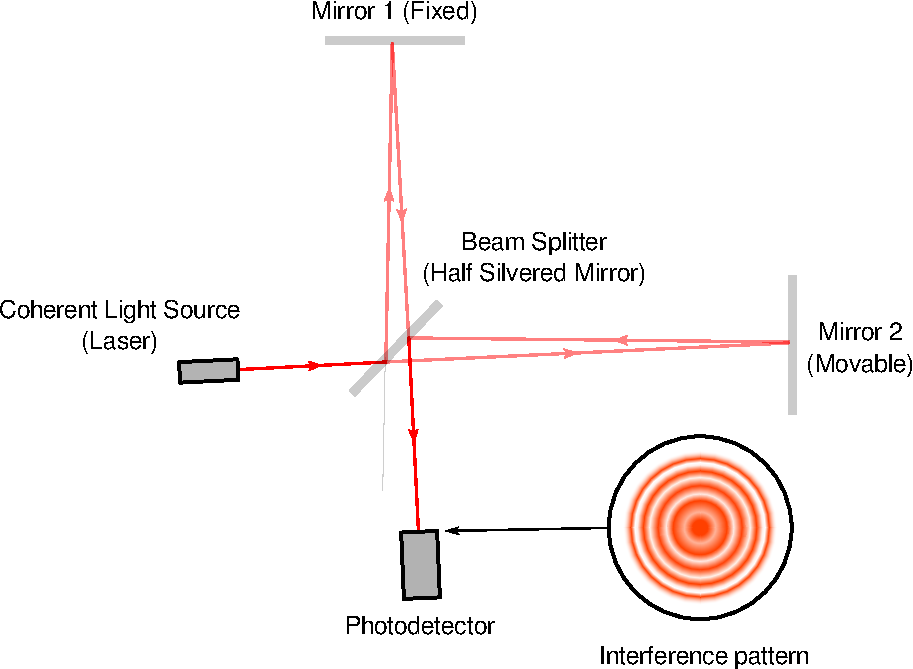
\includegraphics[width=\textwidth]{images/interferometer.pdf}
    \caption{Construction of an Interferometer}
    \label{fig:interferometer}
  \end{subfigure}
  \hspace{25px}
  \begin{subfigure}[t]{0.25\textwidth}
    \centering
    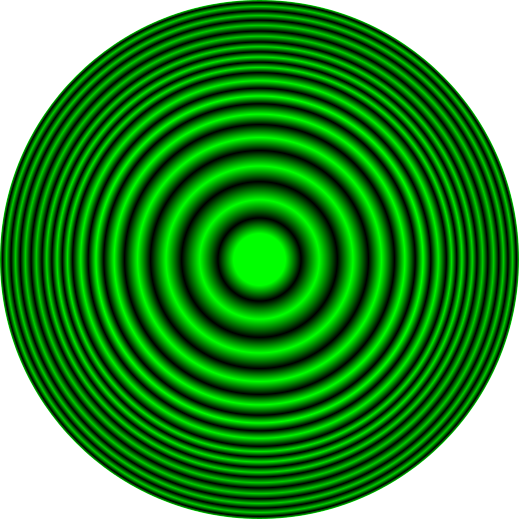
\includegraphics[width=\textwidth]{images/interference_pattern.png}
    \caption{Interference pattern}
    \label{fig:sinusoidal_fringes}
  \end{subfigure}
  \caption{Illustrations of a basic Michelson interferometer \cite{Stannered_Interferometer_2007,wiredsense_michelson_guide} and what an interference pattern would look like.}
\end{figure}

\noindent The \texttt{GWpy} Python package is widely used in this project. It provides a sute of tools to access and condition detector strain data from the Gravitational-Wave Open Science Centre (GWOSC) database \cite{gwpy}. This data is in the time domain, as timestamps in the GPS time system at nanosecond precision, and records the amplitude of the noise event as a differential change in lengths of the interferometer arms. GWpy handles detector data using the \texttt{TimeSeries} object, which is built upon \texttt{numpy} arrays. This allows compatibility with most of the core numpy utilities along with custom functions for signal processing, tabular data filtering, and visualization.

\medskip
\noindent We use the strain data from LIGO Livingston (L1) during the first part of the third observing run (O3a) for this project due to the high rate of occurrence of glitches. Figure \ref{fig:data_acq_cond} shows the steps taken to acquire signal data from the detector and condition it for statistical testing.

\begin{figure}[H]
    \centering
    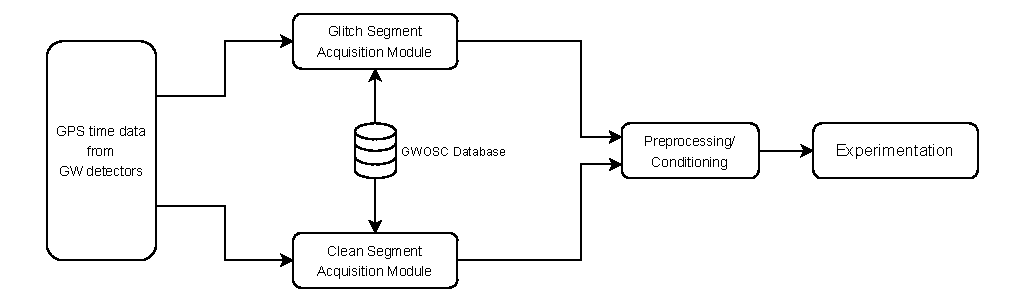
\includegraphics[width=\textwidth]{images/data_acquisition_preparation.pdf}
    \caption{The Data Acquisition and Conditioning Pipeline}
    \label{fig:data_acq_cond}
\end{figure}

\medskip
\noindent There are two main types of detector samples that we receive from the detectors: \textbf{Glitched detector data} and \textbf{Clean detector data}. The following sections will go a bit deeper into each of these types of data and how they are obtained.
  
\subsection{Glitch data}

\medskip
\noindent The GPS times of glitch occurrences are obtained using \textit{Gravity Spy} \cite{Zevin_2017}, a large-scale citizen-science project that combines astrophysics, machine learning, and human efforts to classify glitches in GW interferometer data. The \textit{Omicron} transient search algorithm is used by Gravity Spy to generate q-transform spectrograms and calculate SNR of the time series samples \cite{robinet_omicron_2020}. This algorithm is crucial in identifying the most useful samples for data classification and analysis. Based on the morphological characteristics from the spectrograms, a total of 22 glitch classes were identified with an SNR above 7.5 and peak frequencies between 10 Hz and 2048 Hz.

\medskip
\noindent In the O3a data for L1, Fast\_Scattering and Tomte glitches are the most prevalent, while Chirp, 1080Lines and Wandering\_line glitches have fewer samples, as shown in Table \ref{tab:glitch_classes}. The No\_Glitch class represents glitch samples that lack significant traits or energy levels and do not fit in with the other classes morphologically. Hence, for our study, we do not consider this glitch class.

% \noindent\makebox[\textwidth]{%
\begin{table}[H]
    \centering
    \begin{tabular}{lr|lr}
    \toprule
    Glitch Class & Count & Glitch Class & Count \\
    \midrule
    Fast\_Scattering & 21749 & Whistle & 896 \\
    Tomte & 18708 & Low\_Frequency\_Lines & 788\\
    Blip\_Low\_Frequency & 7549 & Scratchy & 207 \\
    Scattered\_Light & 5398 & Repeating\_Blips & 164 \\
    No\_Glitch & 5358 & Violin\_Mode & 164 \\
    Extremely\_Loud & 4319 & Paired\_Doves & 155 \\
    Koi\_Fish & 4268 & Light\_Modulation & 72 \\
    1400Ripples & 2363 & Helix & 21 \\
    Blip & 1947 & Wandering\_Line & 20 \\
    Power\_Line & 1189 & 1080Lines & 9 \\
    Low\_Frequency\_Burst & 1187 & Chirp & 6 \\
    \bottomrule
    \end{tabular}
    \caption{Glitch counts per class for LIGO Livingston (L1) during the O3a run.}
    \label{tab:glitch_classes}
\end{table}

\pagebreak
\noindent Using the glitch GPS times, the time series information is obtained from the GWOSC database using the \texttt{TimeSeries.fetch\_open\_data()} API provided by GWpy. Here, a time window of 10 seconds is taken on either side of each of the GPS times with the glitch in the center, sampled at a rate of 4096 Hz. The TimeSeries objects obtained are then conditioned for statistical testing and cropped down to a 1-second sample for further use.

\subsection{Clean Samples}

\noindent The process of finding gaps of clean detector noise is done using \texttt{gwtrigfind}, a package developed to search for event triggers files from GW detectors, in conjunction with \texttt{EventTable}, provided by GWpy.

\medskip
\noindent Taking the start and end GPS times of the O3a run, gwtrigfind is used to find the file path containing Omicron triggers from the \textit{L1:GDS-CALIB\_STRAIN} channel of the L1 detector. EventTable is then used to load all the trigger data, containing information on the start and end GPS times of the events. Taking the time frames between the end and start times of successive events, we obtain the gaps between glitches/GW triggers, which do not have a significant amount of noise activity. The sizes of the gaps are clamped between 7 and 30 seconds because too short of a gap could lead to the inclusion of glitches in the sample, as the time series data may not have enough time to stabilize after a glitch; and too long of a time gap could be indicative of detector malfunction or a period of time when it is not operational.

\medskip
\noindent The GPS start and end times of the clean segments are then used to calculate their Q-transform and corresponding p-values. The GPS time intervals with a p-value greater than 0.95 are considered to be clean segments of data, and are used to obtain the corresponding TimeSeries data from GWpy. The TimeSeries data is then, similar to the glitch data, conditioned for statistical testing and cropped down to 1-second samples for further use.


\subsection{Data Conditioning}

\noindent The strain readings obtained from a GW detector is usually a combination of the GW signal and detector noise. In most cases, the noise in the GW detectors is stationary \cite{collaboration_characterization_2016}, i.e. the characteristics of the noise do not change over time, hence keeping the statistical properties constant. However, this is not the case with glitches. Glitches, as discussed in the introduction (\ref{Introduction}) are transient, non-Stationary, non-Gaussian events caused by various environmental factors. These can occur at any time during the observation run and can have a significant impact on the data collected by the detectors. Despite their sources being unknown, they have a large variety of time-frequency morphologies that help characterize them better. During detection runs, glitches show up as short-lived spikes of power in the time series data, increasing the noise floor and affecting the estimation of the power spectral density (PSD) of the data.

\medskip
\noindent The \textbf{Power Spectral Density (PSD)} is a method to represent how power is distributed across different frequencies in a signal \cite{Oppenheim_2009, Li:2013lza}. It is calculated by taking the average of the square of the Fast Fourier transforms (FFT) of the time series data, decomposing the signal into its constituent frequencies. The PSD provides a measure of how much power or strain noise is present at each frequency, allowing for the identification of dominant frequency components and their corresponding amplitudes.

\medskip
\noindent One way to visualize the timeseries data is by using its \textbf{Amplitude Spectral Density (ASD)} values, which are found by taking the square root of the PSD. ASD measures the amplitude of the signal at each frequency, and it is often used to compare the noise levels of different detectors or to assess the a detector's sensitivity to specific frequencies. The ASD is typically plotted on a logarithmic scale, with frequency on the x-axis and ASD on the y-axis, allowing for easy identification of noise peaks and their corresponding frequencies. Figure shows an example

The TimeSeries data obtained from GWpy needs to be conditioned before use for statistical testing.


The two main steps taken for this are \textbf{whitening} and \textbf{filtering}.

\subsubsection{Whitening}

The information obtained from GW detectors encompasses a wide range of frequencies. Due to this, low frequency noise often domainates the data, hence hiding the high frequency components which would be indicative of a signal's presence. Hence, some signal processing is required to counteract this. In Figure \ref{fig:sampletomte} we observe this phenomenon occur in the case of .

\begin{figure}[H]
  \centering
  
\includegraphics[width=0.5\textwidth]{images/sample_plot.pdf}
  \caption{Example of a Tomte glitch with a high SNR. Note that the unwhitened data is dominated by low frequency noise, hence making it difficult to detect the glitch. The whitened data, however, shows a clear peak at the glitch.}
  \label{fig:sampletomte}
\end{figure}

\medskip
\noindent Consider the example of a Tomte glitch 

Whitening is the process of 
\subsubsection{Filtering}

\section{Methods}\label{Methods}
\subsection{Motivation}
\subsection{Shapiro-Wilks Test}
\subsection{KS}
\subsection{AD}
\section{Experimentation with the complete frequency range}\label{Experiment_1}
\section{Experimentation with a band pass filter applied}\label{Experiment_2}
% No of samples, how to recreate the tests we did

% Jarque-Bera test

\section{Conclusions}\label{Conclusions}

\section{Future Scope}\label{Future Scope}

\section{Appendix}\label{Appendix}


% Bibliography
% Acknowledgements
% Appendix

% Describe whitening

% \begin{figure}[H]
%   \centering
%   \begin{subfigure}[t]{0.35\textwidth}
%     \centering
%     \includegraphics[width=\textwidth]{images/me.jpg}
%     \caption{A picture of me}
%     \label{fig:me}
%   \end{subfigure}
%   ~
%   \begin{subfigure}[t]{0.35\textwidth}
%     \centering
%     \includegraphics[width=\textwidth]{images/quantized_me.jpg}
%     \caption{Me, but quantized to a factor of 1}
%     \label{fig:me_quantized}
%   \end{subfigure}
%   \caption{An example of how quantization leads to banding in images}
% \end{figure}


% \begin{minted}[
% frame=lines,
% framesep=2mm,
% baselinestretch=1.2,
% bgcolor=Cornsilk2,
% fontsize=\footnotesize,
% linenos
% ]{Python}
% factor = # An integer factor determined by the user
% for each row from top to bottom:
%     for each column from left to right:
%         oldpixel = image[column][row]

%         # Quantizing the current pixel and calculating the error
%         newpixel = quantize(oldpixel, factor)
%         image[column][row] = newpixel
%         quantization_error = oldpixel - newpixel

%         # Spreading the quantization error to the surrounding pixels
%         image[column+1][row]   = clamp(image[column+1][row]   + (quantization_error*7/16))
%         image[column+1][row+1] = clamp(image[column+1][row+1] + (quantization_error*1/16))
%         image[column][row+1]   = clamp(image[column][row+1]   + (quantization_error*5/16))
%         image[column+1][row-1] = clamp(image[column+1][row-1] + (quantization_error*3/16))

% function quantize(pixel, factor):
%     return round(factor * pixel/255.0) * 255/factor

% # This function prevents the color values from going above 255 or below 0
% function clamp(value):
%     return max(0, min(value, 255))
% \end{minted}

% \begin{figure}[H]
%     \centering
%     \includegraphics[width=0.30\textwidth]{images/RGB_color_gradient_100x100.png}
%     \caption{The Original Image}
%     \label{fig:confirmation_image}
% \end{figure}

% \begin{figure}[h]
%   \centering
%   \begin{subfigure}[t]{0.30\textwidth}
%     \centering
%     \includegraphics[width=\textwidth]{images/dithered_RGB_color_gradient_100x100.png}
%     \caption{Serial Dithering Result}
%     \label{fig:serial_dithering_confirmation}
%   \end{subfigure}
%   ~
%   \begin{subfigure}[t]{0.30\textwidth}
%     \centering
%     \includegraphics[width=\textwidth]{images/parallel_dithered_RGB_color_gradient_100x100.png}
%     \caption{Parallel Dithering Result}
%     \label{fig:parallel_dithering_confirmation}
%   \end{subfigure}
%   \caption{A comparison of the dithering results from our serial and parallel codes.}
% \end{figure}

\printbibliography[title={References}]


\end{document}
